% vim: set tw=78 aw sw=2 sts=2 noet:
\documentclass{beamer}

\usepackage[english]{babel}
\usepackage[utf8x]{inputenc}
\usepackage{comment}
\usepackage{array}
\usepackage{combelow}

\mode<presentation>
{ \usetheme{Rochester} }


\addtobeamertemplate{navigation symbols}{}{%
    \usebeamerfont{footline}%
    \usebeamercolor[fg]{footline}%
    \hspace{1em}%
    \insertframenumber/\inserttotalframenumber
}


\title{Management Styles in IT}
\subtitle{Team Leadership Versus People Management}
\author{Alexandru-George Burghelea \newline
  \textbf{Supervisor}: \cb{S}l. dr. ing. R\u{a}zvan Deaconescu}
  
\begin{document}

\frame{\titlepage}

\begin{frame}{Existing approaches}
Studied management flavors
\begin{description}
\uncover<1->{\item [People Manager] - Soft skilled mentor (3 candidates)} 
\uncover<2->{  \item [Technical Leader] - Coding guru, enforcer (7 candidates)}
\uncover<3->{\item [Team Coach] - Mentor and motivator, mix between PM and TC (4 candidates)}
  
\end{description}
\end{frame}

\iffalse
\begin{frame}{Expectations}
\begin{itemize}
\item Give direction, coordinate, ensure delivery
\item Display commitment, pull their own weight, being flexible and having good technical knowledge
\item Make efforts to improve, be cooperative, be driven towards success
\end{itemize}

\end{frame}
\fi

\begin{frame}{Fear or motivation}
\begin{figure}[h]
  \centering
  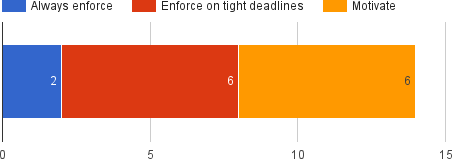
\includegraphics[scale=0.5]{wayofacting.png}
  \caption{Preferred way of acting}
  \label{fig:axbgrid}
\end{figure}

\end{frame}


\begin{frame}{Decision Making (Slackers) }
\begin{figure}[h]
  \centering
  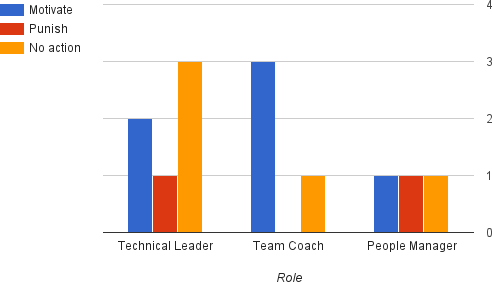
\includegraphics[scale=0.6]{slacker.png}
  \caption{Actions against slackers}
  \label{fig:axbgrid}
\end{figure}
\end{frame}

\begin{frame}{Decision Making (Martyrs)}
\begin{figure}[h]
  \centering
  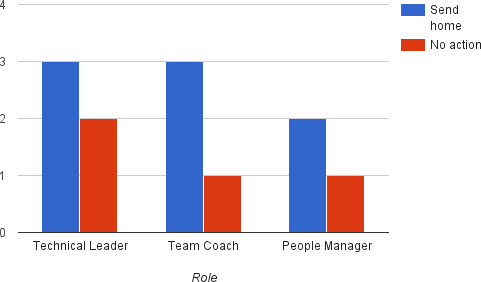
\includegraphics[scale=0.6]{marthyr.png}
  \caption{Actions against martyrs}
  \label{fig:axbgrid}
\end{figure}
\end{frame}

\begin{frame}{Decision Making (part 2)}
\begin{description}
\item[Delegation:] split, prioritize, check candidates, assign
\item[Hiring:] technical background, attitude, expectations
\item[Firing:] no performance, no improvement, no collaboration
\item[Salary adjustment:] evaluate, collect feedback, never announce in advance.
\end{description}
\end{frame}

\begin{frame}{Impediments}
\begin{description}
\uncover<1->{\item[Ego barrier:] over promoting, avoiding risk/members, not admitting mistakes }
\uncover<2->{\item[Nonacceptance of age:] ``You are too young to lead!''}
\uncover<3->{\item[Not addressing problems:] see it, call it, find the cause, feedback}
\end{description}
\end{frame}

\iffalse
\begin{frame}{Ego barrier}
\begin{itemize}
\item over promoting the own person
\item avoiding risks and certain members
\item refusing to admit that they were wrong
\end{itemize}
\end{frame}

\begin{frame}{Not addressing problems}
\begin{itemize}
\item Fail fast
\item See it, call it
\item Understand the cause and fix it, not the effects
\item Track and give feedback
\end{itemize}
\end{frame}
\fi

\begin{frame}{Unofficial Coaching}
\begin{itemize}
\item Try to solve problems by being there
\item Go for a committed language
\item Ask for future plans
\item Try to be there as a colleague
\end{itemize}
\end{frame}

\begin{frame}{Behavioral Coaching}
\begin{itemize}
\item What did you do?
\item What did you expect?
\item What happened?
\item Why do you think it happen that way?
\item How I would have done.
\item What's the plan?
\end{itemize}
\end{frame}

\begin{frame}{Technical Dominance}
\begin{itemize}
\item Come up with a solution
\item No, No, Exactly how I was thinking
\item No, No, No, Solution
\end{itemize}
\end{frame}

\begin{frame}{Conclusion}
\begin{itemize}
\item Be fair, be firm, be honest
\item Treat causes, not effects
\item Give advice only when asked
\item Focus on both people and project
\end{itemize}
\end{frame}

\begin{frame}{Questions}
  \begin{center}
    \bfseries
    \Huge
    ?
  \end{center}
\end{frame}

\end{document}
